% Copyright (c) \hebyear{2025} Dr. Segal Yoram. All rights reserved.
% Comprehensive Template Explanation for hebrew-academic-template.cls
% This document demonstrates ALL available functions with extensive examples

\documentclass{hebrew-academic-template}

% Add bibliography file
\addbibresource{example_references.bib}

% Title page information
\hebrewtitle{מדריך מקיף לשימוש בתבנית האקדמית העברית}
\englishtitle{Comprehensive Guide to Hebrew Academic Template Usage}
\hebrewauthor{ד"ר יורם סגל}

\begin{document}

\maketitle

\tableofcontents
\newpage

% ==================== CHAPTER 1: BASIC USAGE ====================

\hebrewsection{יסודות השימוש בתבנית: Basic Template Usage}

זהו מדריך מקיף לשימוש בתבנית האקדמית העברית \en{hebrew-academic-template.cls}. התבנית תומכת בכתיבה דו-לשונית מתקדמת עם עברית \en{RTL} ואנגלית \en{LTR}, כולל \en{English terms}, ביטויים מתמטיים כמו $E = mc^2$, וכל הפונקציונליות הנדרשת למסמך אקדמי מקצועי.

התבנית כוללת את התכונות הבאות:
- תמיכה מלאה בכיוונים עברית \en{RTL} ואנגלית \en{LTR}
- מספור כותרות ועמודים ב-\en{LTR}
- מספור עמודים ב-\en{LTR}
- תמיכה בטבלאות עם תוכן מעורב
- רשימת מקורות ב-\en{IEEE} סטנדרט
- כותרות עליונות ותחתונות מותאמות
- תמיכה בקוד \en{Python} עם רקע אפור בהיר

\hebrewsubsection{הגדרת המסמך: Document Setup}

כדי להתחיל להשתמש בתבנית:

\begin{pythonbox}[הגדרת המסמך הבסיסית]
\documentclass{hebrew-academic-template}

% Add bibliography file
\addbibresource{references.bib}

% Title page information
\hebrewtitle{כותרת בעברית}
\englishtitle{English Title}
\hebrewauthor{ד"ר שם המחבר}

\begin{document}
\maketitle
\tableofcontents
\newpage
\end{pythonbox}

% ==================== CHAPTER 2: TITLE AND SECTION COMMANDS ====================

\hebrewsection{פקודות כותרות וחלוקה: Title and Section Commands}

\hebrewsubsection{כותרות ראשיות: Main Titles}

התבנית מספקת פקודות מתקדמות ליצירת כותרות עם מספור \en{LTR} וטקסט מעורב:

\begin{pythonbox}[פקודות כותרות ראשיות]
% Hebrew section with LTR numbering
\hebrewsection{שם הפרק בעברית עם English Terms}

% English section with LTR numbering
\englishsection{English Section Title}

% Mixed title function
\HebrewTitle{1}{המרחב הנסתר של ה-AI: The Hidden Space}
\end{pythonbox}

\hebrewsubsection{כותרות משנה: Subsections}

\begin{pythonbox}[פקודות כותרות משנה]
% Hebrew subsection
\hebrewsubsection{כותרת משנה בעברית עם English Integration}

% Manual subtitle creation
\HebrewSubtitle{2.1}{אופטימיזציה: Optimization Methods}
\end{pythonbox}

\hebrewsubsection{דוגמאות כותרות מעורבות: Mixed Title Examples}

\HebrewTitle{3.1}{רגרסיה ליניארית: Linear Regression Fundamentals}

\HebrewTitle{3.2}{אלגוריתמי למידה: Machine Learning Algorithms}

\HebrewTitle{3.3}{ניתוח נתונים: Data Analysis with Python}

% ==================== CHAPTER 3: TEXT DIRECTION AND LANGUAGE SWITCHING ====================

\hebrewsection{כיוון טקסט ומעבר בין שפות: Text Direction and Language Switching}

\hebrewsubsection{פקודות כיוון טקסט: Text Direction Commands}

התבנית מספקת פקודות נוחות למעבר בין שפות וכיוונים:

\begin{pythonbox}[פקודות כיוון וחלפת שפות]
% Short language switching commands
\en{English text}     % English LTR
\heb{טקסט עברי}       % Hebrew RTL
\ilm{inline math}     % Inline math/English terms

% Text direction commands
\LTR{Left-to-Right text}
\RTL{טקסט מימין לשמאל}

% Number formatting in Hebrew text
\num{123}             % Numbers in LTR
\hebyear{2025}        % Years in LTR
\end{pythonbox}

\hebrewsubsection{דוגמאות שימוש מעורב: Mixed Usage Examples}

טקסט עברי עם מספרים \num{100} ושנים \hebyear{2023}, כולל מונחים באנגלית כמו \en{Machine Learning} ו-\en{Deep Learning}. ניתן גם לכלול ביטויים מתמטיים כמו $f(x) = ax^2 + bx + c$ בתוך הטקסט העברי.

בשנת \hebyear{2013} פותח המודל \en{Word2Vec} על ידי \en{Mikolov et al.} \cite{mikolov2013}, שהפך לבסיס לרבים מהמודלים המתקדמים בתחום \en{Natural Language Processing}.

המחקר כולל \num{1000} דגימות מ-\num{50} מדינות שונות, עם דיוק של \num{95.7}\% בבדיקות הביצועים.

% ==================== CHAPTER 4: MATHEMATICAL EXPRESSIONS ====================

\hebrewsection{ביטויים מתמטיים: Mathematical Expressions}

\hebrewsubsection{נוסחאות בסיסיות: Basic Formulas}

התבנית תומכת בביטויים מתמטיים ב-\en{LTR} בתוך טקסט עברי:

משוואת הרגרסיה הליניארית הבסיסית:
\begin{equation}
y = \beta_0 + \beta_1 x_1 + \beta_2 x_2 + \ldots + \beta_n x_n + \varepsilon
\end{equation}

פונקציית העלות \en{(Cost Function)}:
\begin{equation}
J(\theta) = \frac{1}{2m} \sum_{i=1}^{m}(h_\theta(x^{(i)}) - y^{(i)})^2
\end{equation}

\hebrewsubsection{נוסחאות מתקדמות: Advanced Formulas}

אלגוריתם \en{Gradient Descent}:
\begin{equation}
\theta_j := \theta_j - \alpha \frac{\partial}{\partial \theta_j} J(\theta)
\end{equation}

מטריצת הקורלציה:
\begin{equation}
R = \begin{pmatrix}
1 & r_{12} & r_{13} & \cdots & r_{1n} \\
r_{21} & 1 & r_{23} & \cdots & r_{2n} \\
\vdots & \vdots & \ddots & \ddots & \vdots \\
r_{n1} & r_{n2} & r_{n3} & \cdots & 1
\end{pmatrix}
\end{equation}

% ==================== CHAPTER 5: LISTS AND BULLETS ====================

\hebrewsection{רשימות ותבליטים: Lists and Bullets}

\hebrewsubsection{רשימות בסיסיות: Basic Lists}

התבנית תומכת ברשימות עם תוכן מעורב:

רשימת אלגוריתמי למידה:
\begin{itemize}
\item רגרסיה ליניארית: \en{Linear Regression}
\item רגרסיה לוגיסטית: \en{Logistic Regression}  
\item עצי החלטה: \en{Decision Trees}
\item יערות אקראיים: \en{Random Forests}
\item מכונות וקטור תמיכה: \en{Support Vector Machines (SVM)}
\item רשתות נוירונים: \en{Neural Networks}
\end{itemize}

\hebrewsubsection{רשימות ממוספרות: Numbered Lists}

שלבי פיתוח מודל \en{Machine Learning}:
\begin{enumerate}
\item איסוף נתונים: \en{Data Collection}
\item ניקוי נתונים: \en{Data Cleaning}
\item הכנת תכונות: \en{Feature Engineering}
\item בחירת מודל: \en{Model Selection}
\item אימון המודל: \en{Model Training}
\item הערכת ביצועים: \en{Performance Evaluation}
\item פריסה לייצור: \en{Production Deployment}
\end{enumerate}

\hebrewsubsection{רשימות מקוננות: Nested Lists}

סיווג אלגוריתמי למידה:
\begin{itemize}
\item למידה מפוקחת: \en{Supervised Learning}
  \begin{itemize}
  \item רגרסיה: \en{Regression}
    \begin{itemize}
    \item רגרסיה ליניארית: \en{Linear Regression}
    \item רגרסיה פולינומית: \en{Polynomial Regression}
    \end{itemize}
  \item סיווג: \en{Classification}
    \begin{itemize}
    \item \en{k-NN: k-Nearest Neighbors}
    \item \en{SVM: Support Vector Machines}
    \end{itemize}
  \end{itemize}
\item למידה לא מפוקחת: \en{Unsupervised Learning}
  \begin{itemize}
  \item קיבוץ: \en{Clustering}
  \item הפחתת ממדים: \en{Dimensionality Reduction}
  \end{itemize}
\end{itemize}

% ==================== CHAPTER 6: TABLES ====================

\hebrewsection{טבלאות: Tables}

\hebrewsubsection{טבלאות בסיסיות: Basic Tables}

התבנית תומכת בטבלאות עם תוכן מעורב עברית ואנגלית:

\begin{hebrewtable}[h]
\caption{השוואת אלגוריתמי למידה: Comparison of Learning Algorithms}
\begin{rtltabular}{|c|c|c|c|}
\hline
\textbf{אלגוריתם} & \textbf{Algorithm} & \textbf{דיוק} & \textbf{Accuracy} \\
\hline
רגרסיה ליניארית & Linear Regression & \num{85.2}\% & \num{85.2}\% \\
\hline
עץ החלטה & Decision Tree & \num{78.9}\% & \num{78.9}\% \\
\hline
יער אקראי & Random Forest & \num{92.1}\% & \num{92.1}\% \\
\hline
\en{SVM} & Support Vector Machine & \num{88.7}\% & \num{88.7}\% \\
\hline
\end{rtltabular}
\end{hebrewtable}

\hebrewsubsection{טבלאות מתקדמות: Advanced Tables}

\begin{hebrewtable}[h]
\caption{פרמטרים של מודלים שונים: Model Parameters Comparison}
\begin{rtltabular}{|c|c|c|c|c|}
\hline
\textbf{מודל} & \textbf{Model} & \textbf{פרמטרים} & \textbf{Parameters} & \textbf{זמן אימון} \\
\hline
\mixedcell{רגרסיה ליניארית\\Linear Regression} & \en{LinearRegression()} & \num{10} & \num{10} & \num{0.1} שניות \\
\hline
\mixedcell{יער אקראי\\Random Forest} & \en{RandomForest(n=100)} & \num{1000} & \num{1000} & \num{5.2} שניות \\
\hline
\mixedcell{רשת נוירונים\\Neural Network} & \en{MLPRegressor()} & \num{50000} & \num{50000} & \num{45.8} שניות \\
\hline
\end{rtltabular}
\end{hebrewtable}

% ==================== CHAPTER 7: CODE BLOCKS ====================

\hebrewsection{בלוקי קוד: Code Blocks}

\hebrewsubsection{קוד \en{Python} בסיסי: Basic Python Code}

התבנית כוללת סביבת קוד מתקדמת עם רקע אפור בהיר וכיוון \en{LTR}:

\begin{pythonbox}[דוגמה לרגרסיה ליניארית]
import numpy as np
from sklearn.linear_model import LinearRegression
from sklearn.model_selection import train_test_split
from sklearn.metrics import mean_squared_error, r2_score

# Generate sample data
X = np.random.randn(1000, 5)
y = 2*X[:, 0] + 3*X[:, 1] - X[:, 2] + 0.5*X[:, 3] + np.random.randn(1000)*0.1

# Split the data
X_train, X_test, y_train, y_test = train_test_split(X, y, test_size=0.2, random_state=42)

# Create and train the model
model = LinearRegression()
model.fit(X_train, y_train)

# Make predictions
y_pred = model.predict(X_test)

# Evaluate the model
mse = mean_squared_error(y_test, y_pred)
r2 = r2_score(y_test, y_pred)

print(f"Mean Squared Error: {mse:.4f}")
print(f"R-squared Score: {r2:.4f}")
\end{pythonbox}

% ==================== CHAPTER 8: FIGURES AND IMAGES ====================

\hebrewsection{תמונות ואיורים: Figures and Images}

\hebrewsubsection{הוספת תמונות: Adding Images}

התבנית תומכת בהוספת תמונות עם כיתובים מעורבים:

\hebrewfigure[h]{
    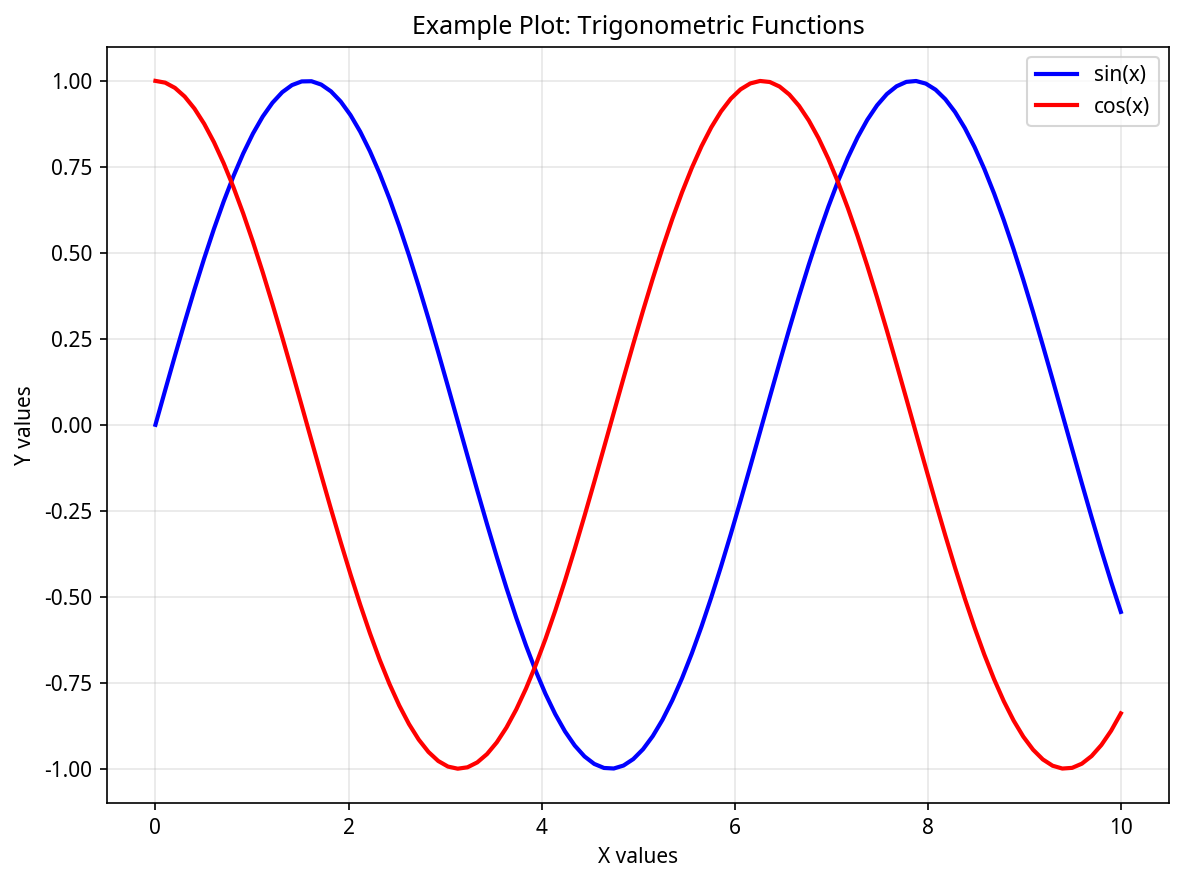
\includegraphics[width=0.6\textwidth]{example_plot.png}
}{
    איור \num{1}: זהו תיאור התמונה בעברית עם English Description - גרף הדגמה
}

% ==================== CHAPTER 9: CITATIONS AND REFERENCES ====================

\hebrewsection{ציטוטים ומקורות: Citations and References}

\hebrewsubsection{ציטוטים בטקסט: In-text Citations}

התבנית תומכת בציטוטים עם מספור \en{LTR} בסגנון \en{IEEE}:

המחקר של \en{Mikolov et al.} \cite{mikolov2013} הציג את מודל \en{Word2Vec} שהפך לבסיס לרבים מהמודלים המתקדמים. מחקרים נוספים \cite{kingma2013,goodfellow2014} הרחיבו את הגישה לתחומים נוספים.

בתחום הרגרסיה הליניארית, העבודה הקלאסית של \en{Galton} \cite{galton1886} הניחה את היסודות לפיתוחים מאוחרים יותר.

\hebrewsubsection{ציטוטים מרובים: Multiple Citations}

מספר מחקרים \cite{mikolov2013,kingma2013,goodfellow2014} הראו את היעילות של שיטות למידה עמוקה בבעיות שונות. התוצאות מצביעות על שיפור משמעותי בביצועים בהשוואה לשיטות מסורתיות \cite{galton1886}.

% ==================== CHAPTER 10: ADVANCED FEATURES ====================

\hebrewsection{תכונות מתקדמות: Advanced Features}

\hebrewsubsection{הגדרות גופנים: Font Configuration}

התבנית כוללת מנגנון \en{fallback} חכם לגופנים:

\begin{pythonbox}[הגדרות גופנים]
% Windows/MiKTeX fonts (preferred)
Times New Roman    -> Main font
David CLM         -> Hebrew font  
Arial             -> Sans-serif font
Courier New       -> Monospace font

% Linux/TeX Live fallbacks
Latin Modern Roman -> Main font fallback
DejaVu Sans       -> Hebrew font fallback
Latin Modern Sans -> Sans-serif fallback
DejaVu Sans Mono  -> Monospace fallback
\end{pythonbox}

\hebrewsubsection{פקודות עזר: Utility Commands}

\begin{pythonbox}[פקודות עזר נוספות]
% Inline code
\code{variable_name}

% English terms in Hebrew text
\englishterm{Machine Learning}

% Hebrew figures
\hebrewfigure[h]{content}{caption}

% Mixed cell content in tables
\mixedcell{עברית\\English}
\hebcell{עברית בלבד}
\end{pythonbox}

% ==================== CHAPTER 11: COMPLETE EXAMPLE ====================

\hebrewsection{דוגמה מלאה: Complete Example}

\hebrewsubsection{מסמך מלא: Full Document Example}

\begin{pythonbox}[מבנה מסמך מלא]
\documentclass{hebrew-academic-template}
\addbibresource{references.bib}

\hebrewtitle{כותרת המחקר בעברית}
\englishtitle{Research Title in English}
\hebrewauthor{ד"ר שם החוקר}

\begin{document}
\maketitle
\tableofcontents
\newpage

\hebrewsection{מבוא: Introduction}
טקסט המבוא עם ציטוטים \cite{reference1} ומונחים באנגלית \en{Machine Learning}.

\hebrewsubsection{מתודולוגיה: Methodology}
תיאור השיטות עם נוסחאות:
\begin{equation}
y = \beta_0 + \beta_1 x + \varepsilon
\end{equation}

\begin{pythonbox}[קוד לניתוח]
import pandas as pd
data = pd.read_csv('data.csv')
print(data.head())
\end{pythonbox}

\hebrewsection{תוצאות: Results}
הצגת התוצאות בטבלה:

\begin{hebrewtable}[h]
\caption{תוצאות הניסוי: Experimental Results}
\begin{rtltabular}{|c|c|c|}
\hline
\textbf{מדד} & \textbf{Metric} & \textbf{ערך} \\
\hline
דיוק & Accuracy & \num{95.2}\% \\
\hline
\end{rtltabular}
\end{hebrewtable}

\hebrewsection{מסקנות: Conclusions}
סיכום המחקר והמלצות להמשך.

% Bibliography
\newpage
\printenglishbibliography

\end{document}
\end{pythonbox}

% ==================== BIBLIOGRAPHY ====================

\newpage
\printenglishbibliography

\end{document}
